\documentclass[compress,aspectratio=43]{beamer}
\usepackage[latin1]{inputenc}
\usepackage{tikz}
\usepackage{xcolor}
\usepackage{amsmath,amssymb,epsfig,graphicx,url,bbm,epstopdf}

%\usetheme{Szeged}
\useoutertheme[subsection=false, footline=institutetitle]{miniframes}
\usecolortheme{beaver}

\setbeamercolor{subtitle}{fg=black} % Change subtitle color
\setbeamercolor{block title}{fg=black} % Change subtitle color
\setbeamercolor{itemize item}{fg=red}
\setbeamercolor{itemize itemize}{fg=red}


\setbeamertemplate{navigation symbols}{}%remove navigation symbols
\definecolor{darkgreen}{rgb}{0,0.5,0}

% Footer
\makeatletter
\setbeamertemplate{footline}
{
  \leavevmode%
  \hbox{%
  \begin{beamercolorbox}[wd=.333333\paperwidth,ht=2.25ex,dp=1ex,left]{section in head/foot}%
    \usebeamerfont{author in head/foot}\insertshortauthor
  \end{beamercolorbox}%
  \begin{beamercolorbox}[wd=.333333\paperwidth,ht=2.25ex,dp=1ex,center]{section in head/foot}%
    \usebeamerfont{title in head/foot}\insertshorttitle
  \end{beamercolorbox}%
  \begin{beamercolorbox}[wd=.333333\paperwidth,ht=2.25ex,dp=1ex,right]{section in head/foot}%
    \usebeamerfont{date in head/foot}\insertshortdate{}\hspace*{2em}
    \insertframenumber{} / \inserttotalframenumber\hspace*{2ex} 
  \end{beamercolorbox}}%
  \vskip0pt%
}
\makeatother

\usebackgroundtemplate{%
	\tikz\node[opacity=0.05] {\includegraphics[height=500px,width=500px]{stanford_seal.png}};
}

% Removes title background bar
\setbeamercolor*{frametitle}{bg=}
\setbeamercolor{titlelike}{parent=structure}

\title[Stanford University]{GrabCut - Interactive Foreground Extraction using Iterated Graph Cuts}
\subtitle{\scriptsize \vspace{3mm}Carsten Rother, Vladimir Kolmogorov, and Andrew Blake\\Microsoft Research Cambridge, UK\vspace{-3mm}}
\author[\enspace\,\,\, Albert Haque, Fahim Dalvi]{
{\scriptsize Project Presentation By}\\
{\small Albert Haque and Fahim Dalvi}\\
\vspace{-6mm}}
\institute[Stanford University]{}
\date{April 20, 2015}
\begin{document}

\section{}% Top left running header
\begin{frame}
\titlepage
\end{frame}

\begin{frame}{Outline}
\begin{itemize}
\item Hyperparameter Tuning
\begin{itemize}
    \item{Neighborhood Size}
    \item{GMM Components}
    \item{Iterations}
\end{itemize}
\item Tight vs Loose Bounding Box
\item User Interaction
\item Entropy-Based Gamma Optimization
\end{itemize}
\end{frame}

\begin{frame}{Hyperparameter Tuning}
\begin{columns}[t]
\column{.3\textwidth}
\centering
{\scriptsize Number of Iterations}\\ \vspace{2mm}
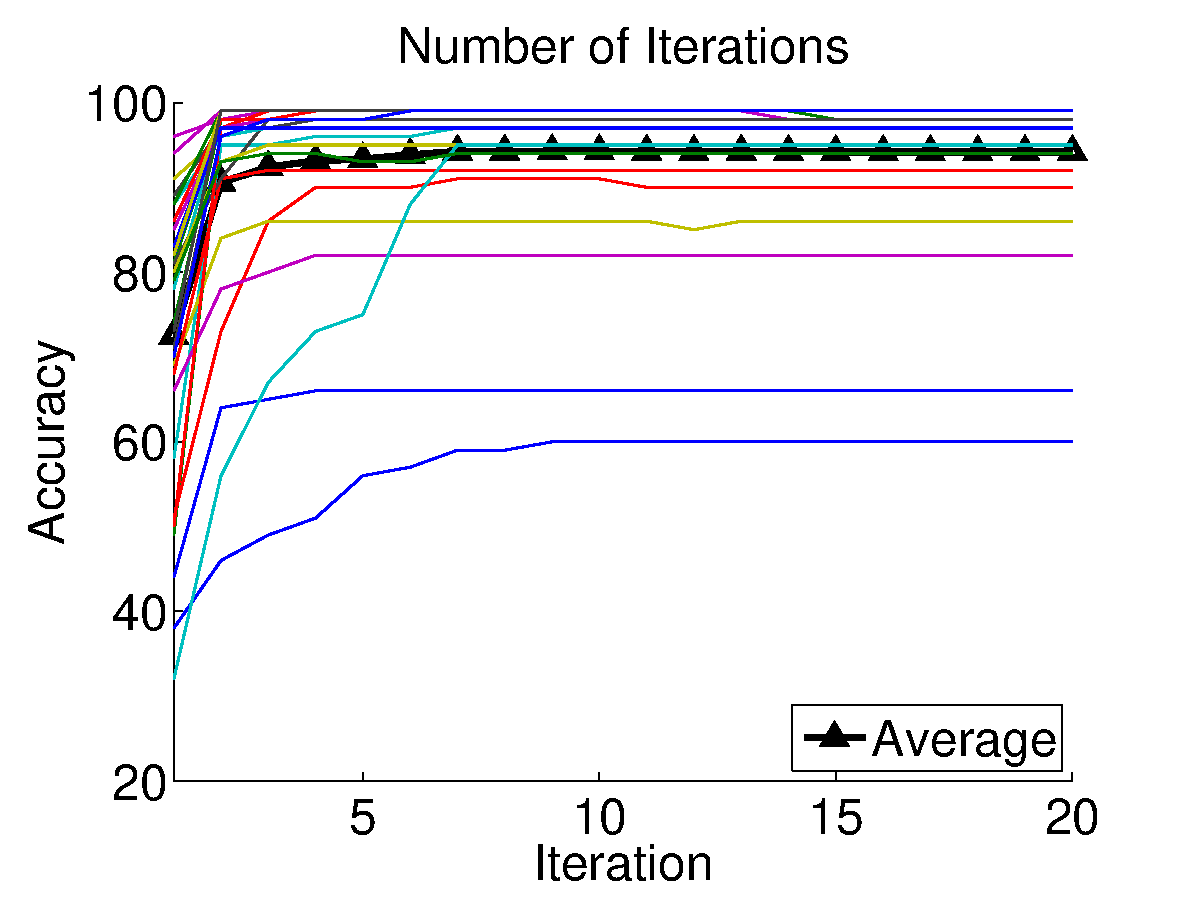
\includegraphics[width=1\linewidth]{figures/hyperparameter_tuning/iterations/accuracy.eps}\\
\includegraphics[width=1\linewidth]{figures/hyperparameter_tuning/iterations/jaccard.eps}\\
{\tiny
At 20 iterations:\\
Accuracy: $94.1 \pm 9.4$\\
\vspace{-2mm}
Jaccard: $82.1 \pm 17.9$
}
\column{.3\textwidth}
\centering
{\scriptsize GMM Components}\\ \vspace{2mm}
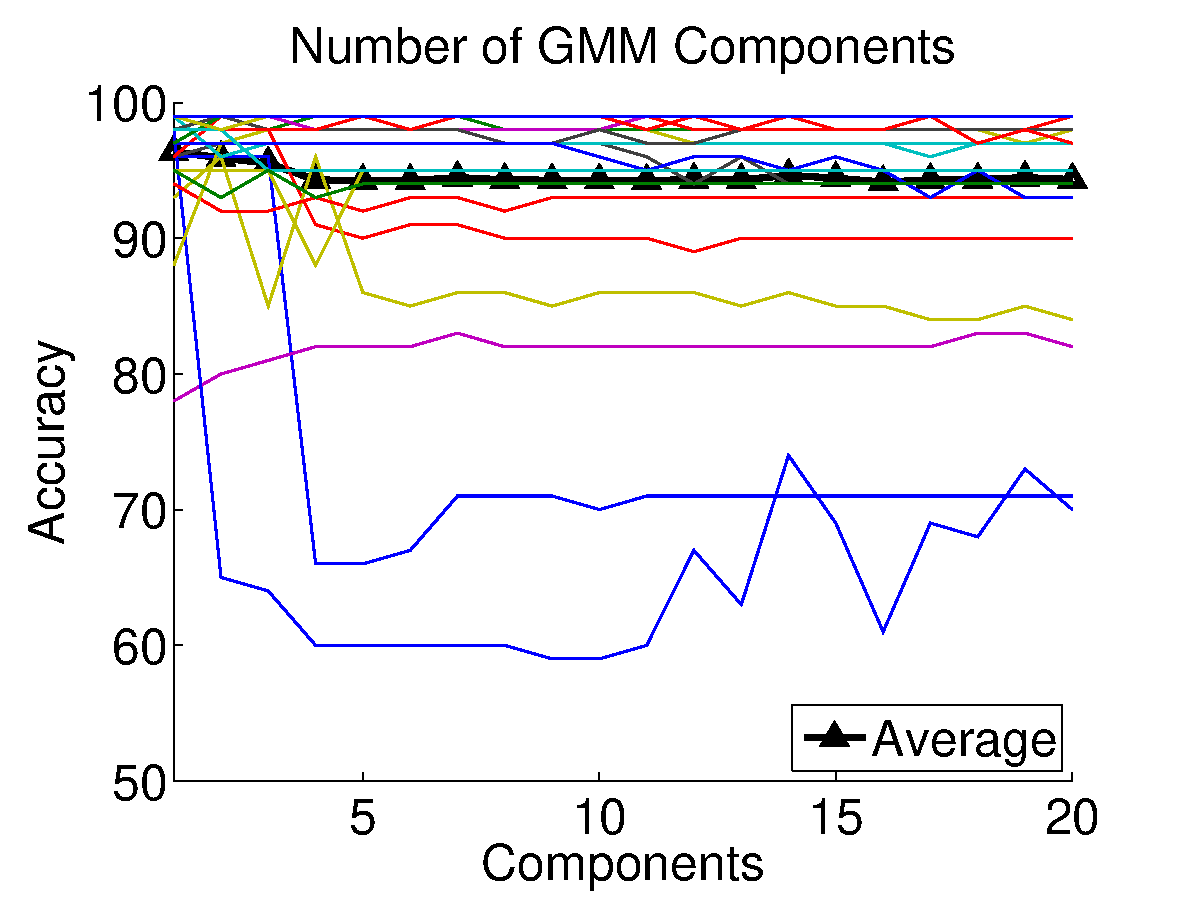
\includegraphics[width=1\linewidth]{figures/hyperparameter_tuning/components/accuracy.eps}\\
\includegraphics[width=1\linewidth]{figures/hyperparameter_tuning/components/jaccard.eps}\\
{\tiny
At 20 components:\\
Accuracy: $94.3 \pm 7.7$\\
\vspace{-2mm}
Jaccard: $81.1 \pm 17.1$
}

\column{.4\textwidth}
\begin{center}
\vspace{-7mm}
{\scriptsize Neighborhood Size}\\
\end{center}
{\scriptsize Four Neighbors}
\begin{itemize}
{\scriptsize 
\item Accuracy: $93.5 \pm 9.2$
\item Jaccard: $80.0 \pm 19.5$
}
\end{itemize}

{\scriptsize Eight Neighbors}
\begin{itemize}
{\scriptsize 
\item Accuracy: $94.2 \pm 9.45$
\item Jaccard: $82.3 \pm 17.9$
}
\end{itemize}
\end{columns}
\end{frame}

\begin{frame}{Tight vs Loose Bounding Box}
\begin{columns}
\uncover<1->{
\column{.2\textwidth}
\centering
\includegraphics[width=1\linewidth]{figures/hyperparameter_tuning/bounding_boxes/cross-bbox.png}\\
\includegraphics[width=1\linewidth]{figures/hyperparameter_tuning/bounding_boxes/doll-bbox.png}\\
\includegraphics[width=1\linewidth]{figures/hyperparameter_tuning/bounding_boxes/elefant-bbox.png}\\
}
\uncover<2->{
\column{.41\textwidth}
\centering
{\scriptsize
\begin{itemize}
\vspace{5px}
\item Cross
\begin{itemize}
{\scriptsize
\item Accuracy: 60\%$\rightarrow${\textbf{\color{red}59\%}}
\item Jaccard: 42\%$\rightarrow${\textbf{\color{red}39\%}}
}
\end{itemize}
\vspace{30px}
\item Doll
\begin{itemize}
{\scriptsize
\item Accuracy: 99\%$\rightarrow$99\%
\item Jaccard: 98\%$\rightarrow$98\%
}
\end{itemize}
\vspace{30px}
\item Elefant
\begin{itemize}
{\scriptsize
\item Accuracy: 92\%$\rightarrow${\textbf{\color{darkgreen}96\%}}
\item Jaccard: 81\%$\rightarrow${\textbf{\color{darkgreen}89\%}}
}
\end{itemize}
\end{itemize}
}
}
\uncover<3->{
\column{.39\textwidth}
\begin{itemize}
{\scriptsize
\item Original bouding boxes
\begin{itemize}
{\scriptsize
\item Accuracy: 94\%
\item Jaccard: 82\%
}
\end{itemize}
\item Tighter bouding boxes
\begin{itemize}
{\scriptsize
\item Accuracy: 95\%
\item Jaccard: 84\%
}
\end{itemize}
}
\end{itemize}
}
\end{columns}
\end{frame}

\begin{frame}{User Interaction}
\begin{columns}[t]
\uncover<1->{
\column{.2\textwidth}
\centering
{\scriptsize Iteration 0}
\includegraphics[width=1\linewidth]{figures/user_interaction/banana/user0_iter1.png}\\
\includegraphics[width=1\linewidth]{figures/user_interaction/bool/user0_iter1.png}
}
\uncover<2->{
\column{.2\textwidth}
\centering
{\scriptsize Iteration 1}
\includegraphics[width=1\linewidth]{figures/user_interaction/banana/user0_iter2.png}\\
\includegraphics[width=1\linewidth]{figures/user_interaction/bool/user0_iter2.png}
}
\uncover<3->{
\column{.2\textwidth}
\centering
{\scriptsize User Interaction}
\includegraphics[width=1\linewidth]{figures/user_interaction/banana/user_interaction.png}\\
\includegraphics[width=1\linewidth]{figures/user_interaction/bool/user_interaction.png}
}
\uncover<4->{
\column{.2\textwidth}
\centering
{\scriptsize Iteration 2}
\includegraphics[width=1\linewidth]{figures/user_interaction/banana/user1_iter1.png}\\
\includegraphics[width=1\linewidth]{figures/user_interaction/bool/user1_iter1.png}
}
\uncover<5->{
\column{.2\textwidth}
\centering
{\scriptsize Segmentation}
\includegraphics[width=1\linewidth]{figures/user_interaction/banana/user1_segmentation.png}\\
\includegraphics[width=1\linewidth]{figures/user_interaction/bool/user1_segmentation.png}
}
\end{columns}
\vspace{-2mm}
\begin{columns}[t]
\uncover<6->{
\column{.5\textwidth}
Before
\begin{itemize}
\item Banana1
\begin{itemize}
\item Accuracy: 66\%
\item Jaccard: 43\%
\end{itemize}
\item Bool
\begin{itemize}
\item Accuracy: 82\%
\item Jaccard: 41\%
\end{itemize}
\end{itemize}
}
\uncover<7->{
\column{.5\textwidth}
After (with user interaction)
\begin{itemize}
\item Banana1
\begin{itemize}
\item Accuracy: 99\%
\item Jaccard: 96\%
\end{itemize}
\item Bool
\begin{itemize}
\item Accuracy: 98\%
\item Jaccard: 87\%
\end{itemize}
\end{itemize}
}
\end{columns}
\end{frame}

\begin{frame}{Entropy-Based Gamma Optimization}
\begin{columns}[t]
\column{.15\textwidth}
\includegraphics[width=1\linewidth]{figures/gamma/banana/banana1-rgb.png}\\
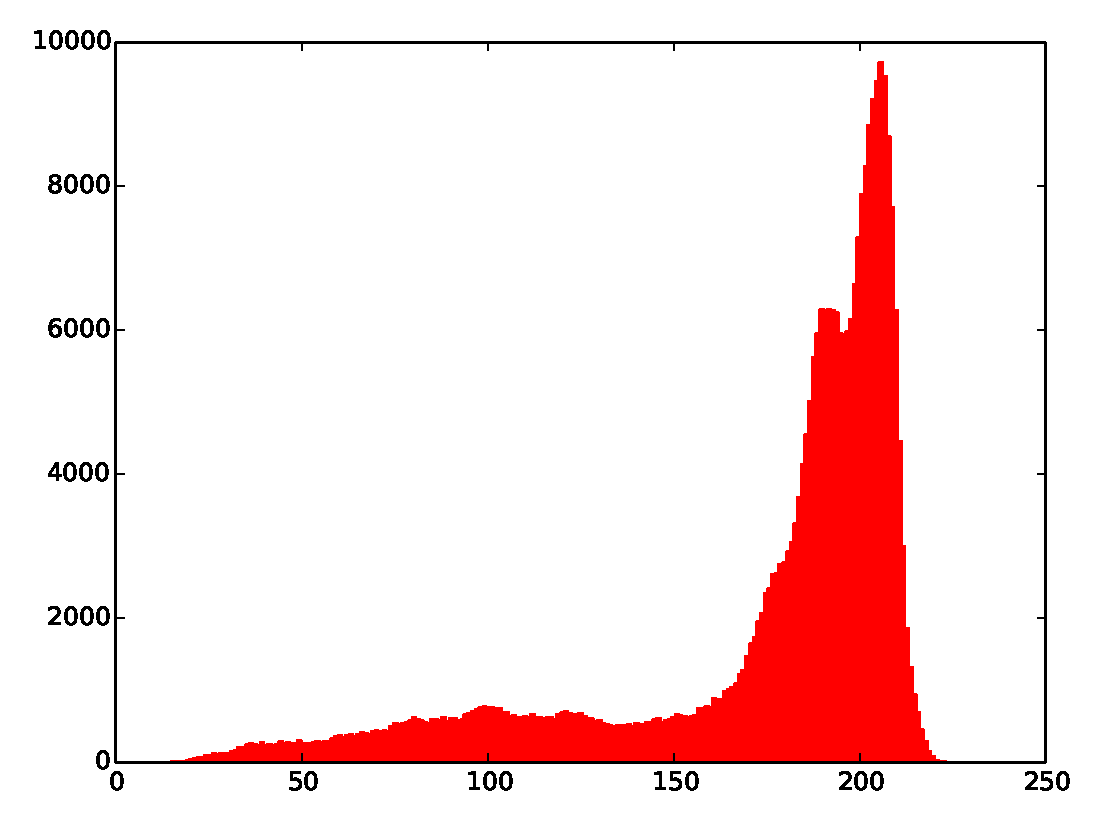
\includegraphics[width=1\linewidth]{figures/gamma/banana/banana1-r.eps}\\
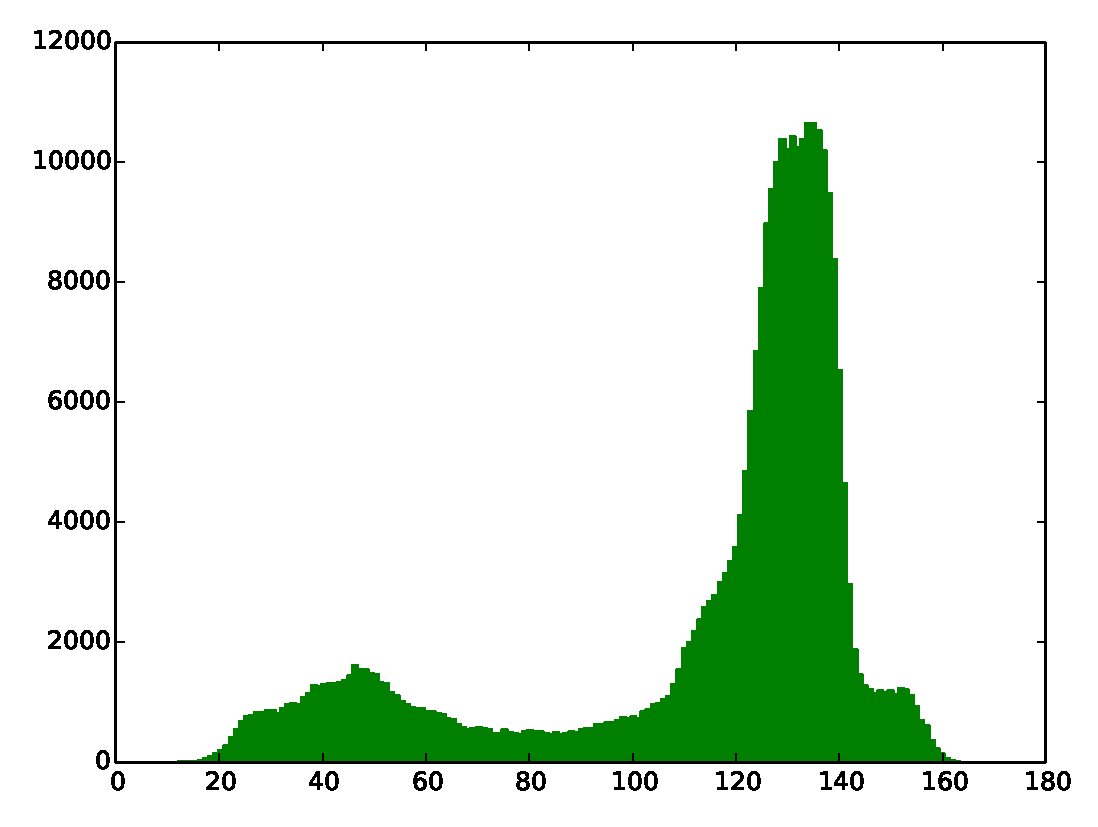
\includegraphics[width=1\linewidth]{figures/gamma/banana/banana1-g.eps}\\
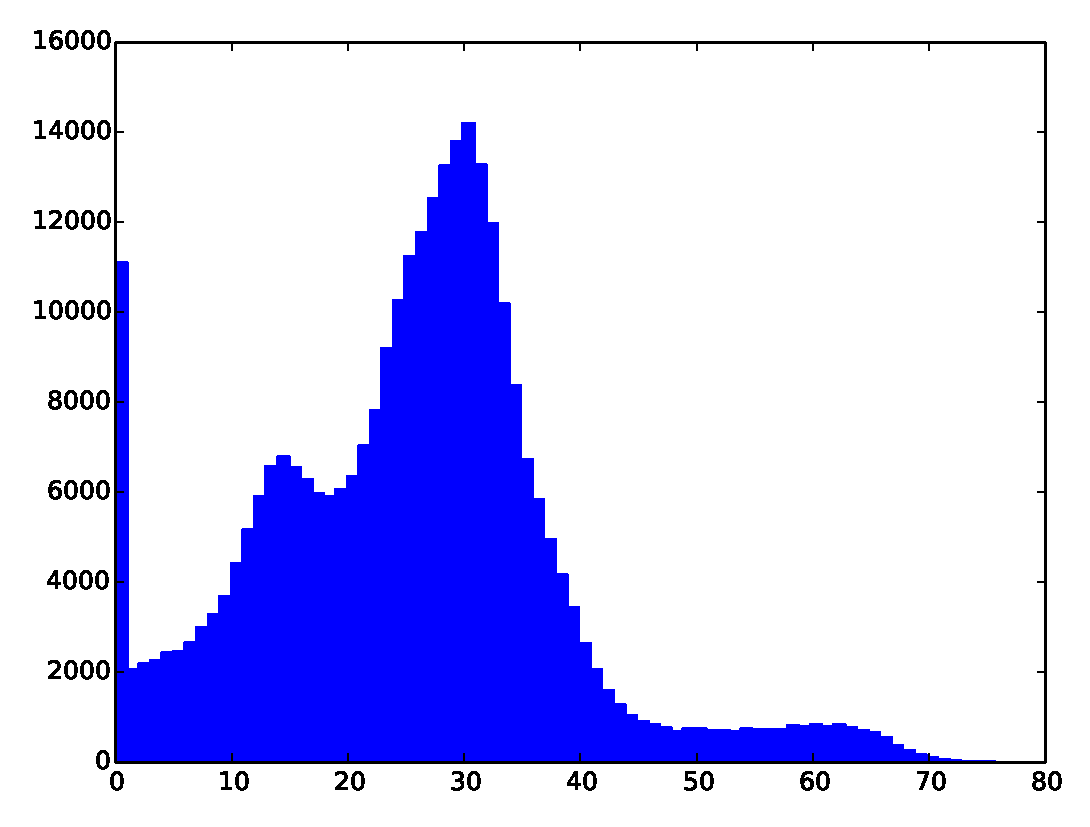
\includegraphics[width=1\linewidth]{figures/gamma/banana/banana1-b.eps}\\
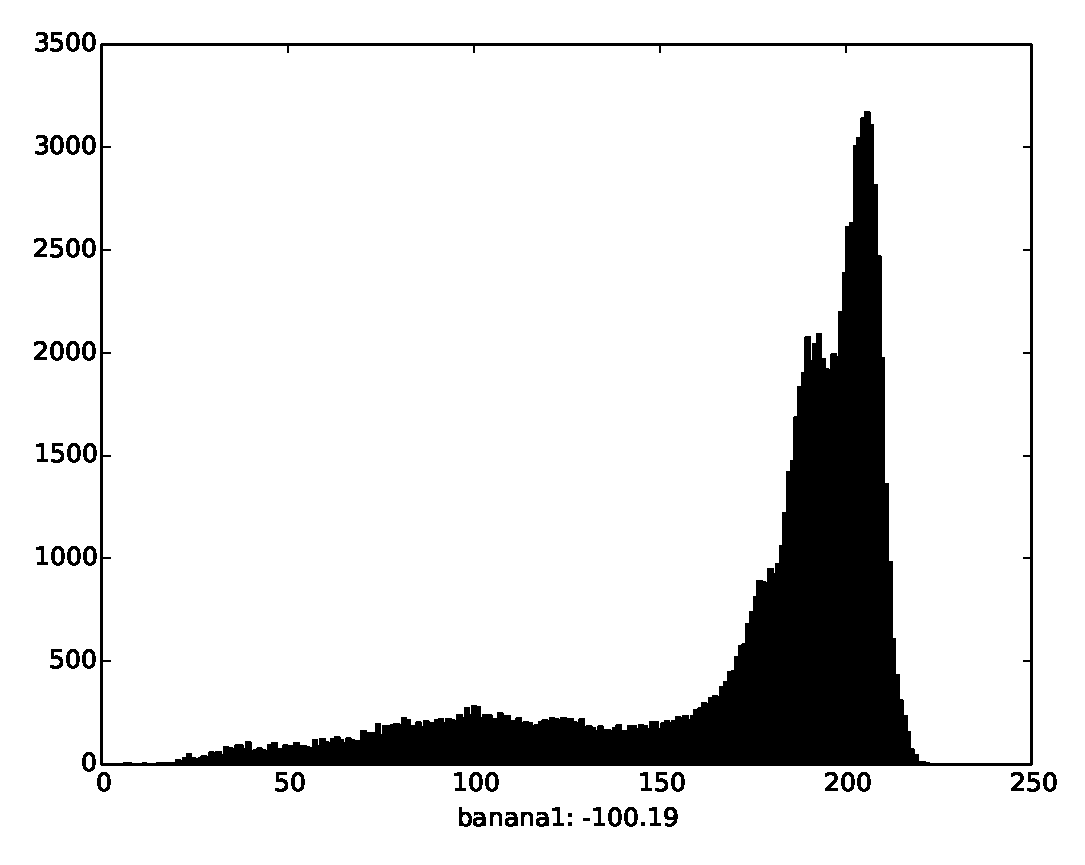
\includegraphics[width=1\linewidth]{figures/gamma/banana/banana1-h.eps}
\column{.15\textwidth}
\includegraphics[width=1\linewidth]{figures/gamma/flower/flower-rgb.png}\\
\includegraphics[width=1\linewidth]{figures/gamma/flower/flower-r.eps}\\
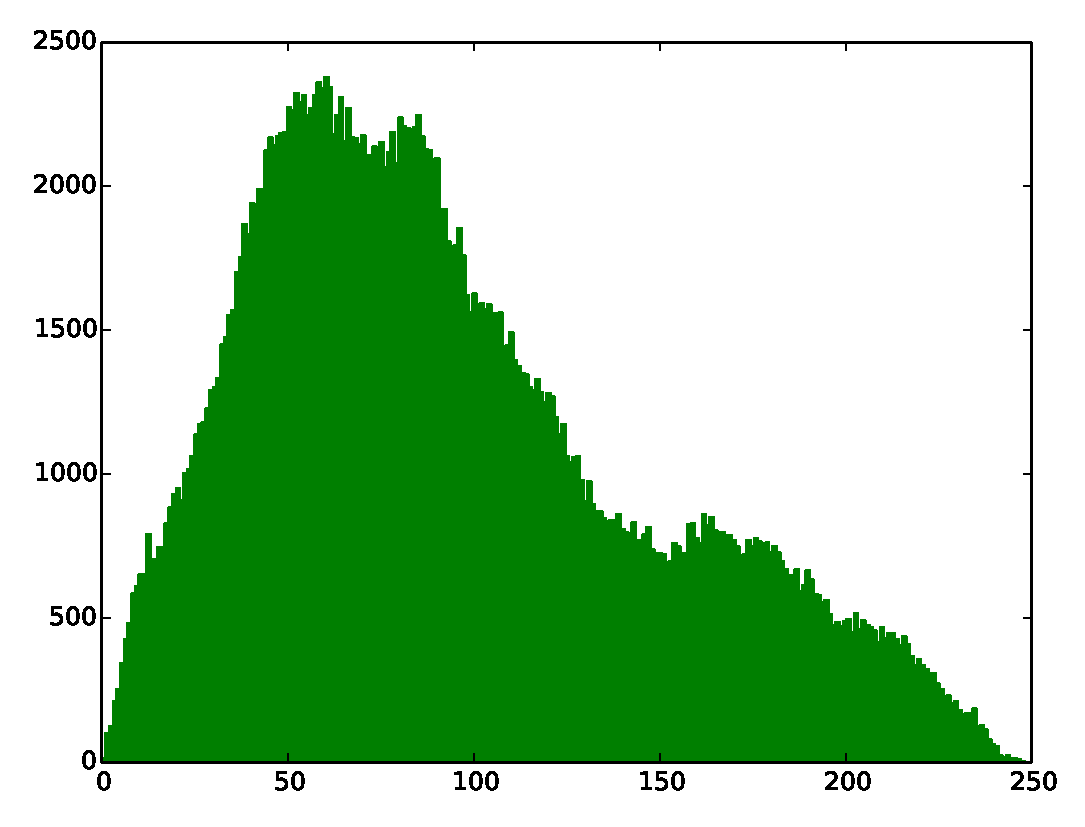
\includegraphics[width=1\linewidth]{figures/gamma/flower/flower-g.eps}\\
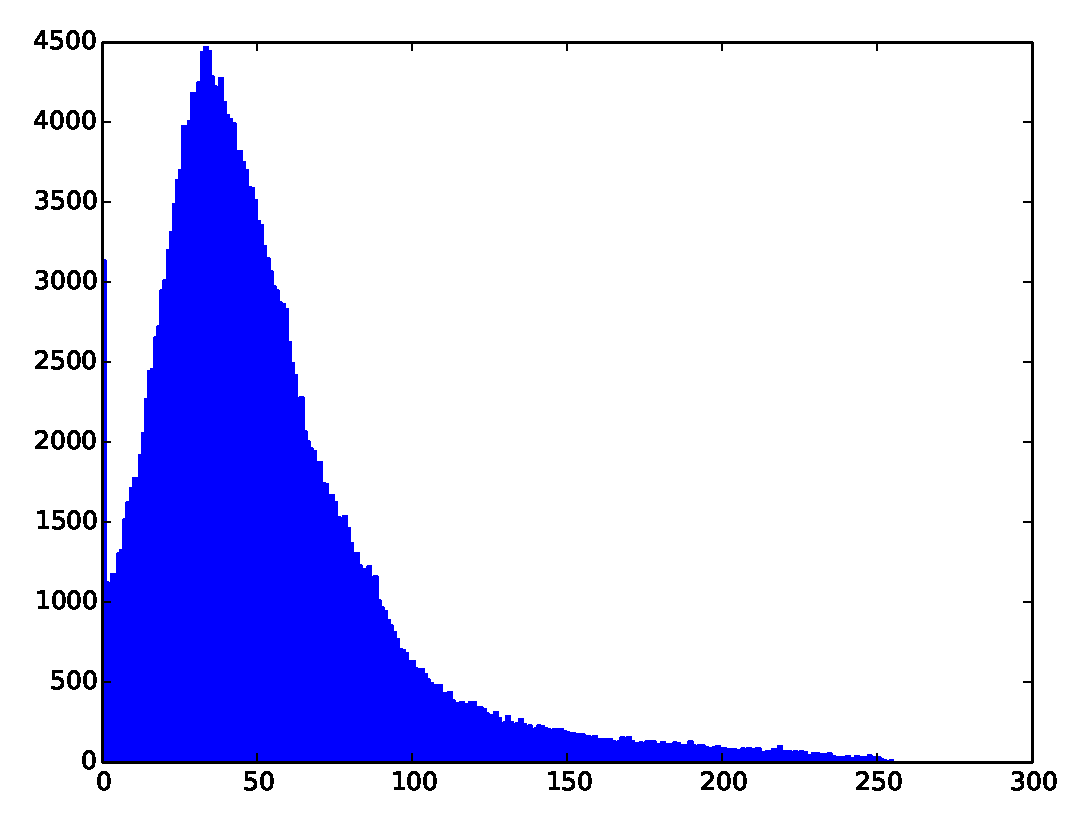
\includegraphics[width=1\linewidth]{figures/gamma/flower/flower-b.eps}\\
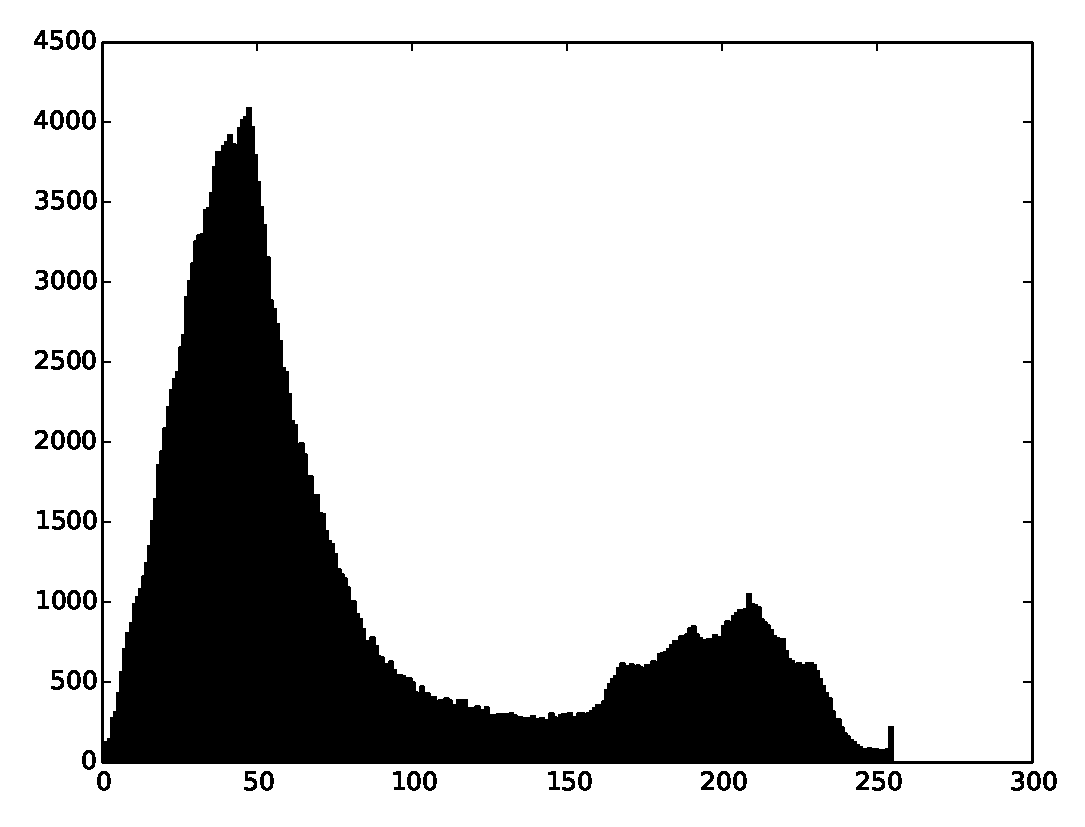
\includegraphics[width=1\linewidth]{figures/gamma/flower/flower-h.eps}
\column{.7\textwidth}
{\scriptsize
Motivation
\begin{itemize}
\item Color-skewed images (e.g. banana1)
\item Unary energies capture color information better than pairwise
\item Pairwise energies should be smaller
\item Reduce gamma for color-skewed images
\end{itemize}

Experiments
\begin{itemize}
\item Reducing gamma results in better segmentation\\
\begin{center}
\includegraphics[width=0.3\linewidth]{figures/gamma/banana1_high_gamma.png}\hspace{5mm}
\includegraphics[width=0.3\linewidth]{figures/gamma/banana1_low_gamma.png}
\end{center}
\item Next: Automate gamma selection based on entropy
\end{itemize}
}
\end{columns}
\end{frame}

\end{document}